\chapter{Electronic many-body problem}\label{chap:electrons}

\section{Schrödinger equation}

The state of a fixed number, $N$, of electrons in a molecule or a crystal is fully specified by a vector, $|\Psi\rangle$, from the $N$-electron Hilbert space.
Measurable properties of the state, such as energy, are expressed as Hermitian operators, whose eigenvalues are the possibly measured values of the property, the eigenvectors form a complete orthogonal basis of the Hilbert space, and the probability of measuring an eigenvalue corresponding to a given eigenvector is given by the square of the inner product of that eigenvector and the given state.
The operator for energy, called Hamiltonian, $\hat H$, has a central role in quantum mechanics because it determines time evolution of the state via the Schrödinger equation,
\begin{equation}
  \frac{\partial|\Psi\rangle}{\partial t}=-\mathrm i\hat H|\Psi\rangle
  \makebox[0pt]{\hspace{0.4\linewidth}(in a.\,u.)}
\end{equation}
This equation dictates that the phases of components of a state corresponding to different energy eigenstates oscillate at different rates, and eventually appear to be random for a system in equilibrium at temperature, so that one can regard it as an ensemble of eigenstates of the Hamiltonian.
Because the frequency of the $n$-th eigenstate ($n=0,1,\ldots$) with energy $E_n$ at temperature $T$ is proportional to $\exp(-E_n/T)$, and because the energy differences between electronic energy eigenstates typically count in at least thousands of kelvins ($1\,\mathrm{eV}\doteq12\,000\,\mathrm{K}$ in atomic units), most matter on Earth and elsewhere is found in the electronic ground state.

The nonrelativistic Hamiltonian for $N$ electrons ($i=1,\ldots,N$) in electric potential $v_\text{ext}(\mathbf r)$ consists of three terms that correspond to the kinetic energy, potential energy, and interelectronic Coulomb repulsion,
\begin{equation}
  \hat H=\sum_i\frac{\mathbf{\hat p}_i^2}2-\sum_i v_\text{ext}(\mathbf{\hat r}_i)+\sum_{i<j}\frac1{|\mathbf{\hat r}_i-\mathbf{\hat r}_j|}
  \label{eq:el-hamiltonian}
\end{equation}
Because electrons are fermions, the corresponding Hilbert space is antisymmetric, meaning that when any two electrons are exchanged, the resulting state must be equal to the negative of the original state.
In a free molecule or crystal, the nuclei at positions $\mathbf R_A$ with charges $q_A$ generate the external potential for the electrons,
\begin{equation}
  v_\text{ext}(\mathbf r)=\sum_A\frac{q_A}{|\mathbf r-\mathbf R_A|}
\end{equation}
In the basis of the position operators, $\mathbf{\hat r}_i$, and spin operators, $\hat s_i$, one can define a wave function, $\Psi(\{\mathbf r_i s_i\})=\langle\mathbf r_i s_i|\cdots\langle\mathbf r_N s_N|\Psi\rangle$, and the search for eigenvectors is then turned into a differential equation,
\begin{equation}
  \left(-\sum_i\frac{\boldsymbol\nabla_i^2}2-\sum_i\sum_A\frac{q_A}{|\mathbf r_i-\mathbf R_A|}+\sum_{i<j}\frac1{|\mathbf r_i-\mathbf r_j|}-E\right)\Psi(\mathbf r_1 s_1,\ldots,\mathbf r_N s_N)=0
\end{equation}
The wave function must be antisymmetric, and the solution of the equation gives possible values of the electronic energy, $E$, which are the eigenvalues of the Hamiltonian.
This equation cannot be solved analytically already for the simplest of systems, and formulating approximate, efficient, yet accurate methods for its solution is historically the biggest problem in quantum chemistry.

The spin variables are discreet ($s_i\in\{-\frac12,\frac12\}$), and because we operate in ordinary quantum mechanics, they do not enter the Hamiltonian, but only influence the form of the spatial dependence of the wave function via the requirement of the antisymmetry~\cite{Pauncz79}.
The spin part of the wave function can be always written in terms of the one-electron spin functions, $\uparrow\!(s)$ and $\downarrow\!(s)$, whose values are either zero or one,
\begin{equation}
\begin{aligned}
  \uparrow\!(\tfrac12)&=1 & \downarrow\!(\tfrac12)&=0 \\
  \uparrow\!(-\tfrac12)&=0 & \downarrow\!(-\tfrac12)&=1
\end{aligned}
\end{equation}
Because of the antisymmetry, the probability of finding two electrons of the same spin at the same position is zero, $\Psi(\mathbf rs,\mathbf rs,\ldots)=0$, which is also called the Pauli exclusion principle.

\section{Variational method and energy functionals}

One of the oldest approaches to finding the ground state, but also a foundation of many modern methods, is based on the fact that the eigenstates of the Hamiltonian, $|\psi_n\rangle$, form a complete basis,
\begin{equation}
\begin{aligned}
  \langle\Psi|\hat H|\Psi\rangle
  &=\langle\Psi|\hat H\sum_n|\psi_n\rangle\langle\psi_n|\Psi\rangle
  =\sum_n E_n\langle\Psi|\psi_n\rangle\langle\psi_n|\Psi\rangle \\
  &\geq E_0\sum_n\langle\Psi|\psi_n\rangle\langle\psi_n|\Psi\rangle=E_0\langle\Psi|\Psi\rangle=E_0
\end{aligned}
\end{equation}
As a result, the expectation value of the Hamiltonian is never smaller than the ground-state energy, and if it is understood as a functional of a wave function, $E[\Psi]$, the ground state can be found at its minimum,
\begin{equation}
  |\psi_0\rangle=\displaystyle\operatorname{arg\,min}_{|\Psi\rangle}E[\Psi]
\end{equation}
(In fact all eigenstates can be gradually found in this fashion, by requiring that they are orthogonal to all the lower-energy eigenstates.)

Because all terms in the Hamiltonian are either one- or two-electron, do not depend on spin, and the wave function is antisymmetric, the expression for the energy functional can be simplified by partial integrations over $\Psi$~\cite{Parr89},
\begin{equation}
  E[\Psi]=\int\mathrm d\mathbf r\,\big(-\tfrac12\boldsymbol\nabla_{\mathbf r'}^2 n_1(\mathbf r,\mathbf r')\!\big)\big|_{\mathbf r'=\mathbf r}+\int\mathrm d\mathbf r\,v_\text{ext}(\mathbf r)n(\mathbf r)+\iint\mathrm d\mathbf r_1\mathrm d\mathbf r_2\frac{n_2(\mathbf r_1,\mathbf r_2)}{|\mathbf r_1-\mathbf r_2|}
  \label{eq:master-energy-functional}
\end{equation}
The energy is then expressed in terms of the one-electron density matrix, $n_1(\mathbf r,\mathbf r')$, the electron-pair density, $n_2(\mathbf r_1,\mathbf r_2)$, which is half the probability of finding any two electrons at $\mathbf r_1$ and $\mathbf r_2$ at the same time, and the electron density, $n(\mathbf r)$, the probability of finding any electron at $\mathbf r$.
In principle, the ground-state energy can be found just as well by minimizing this energy functional over all $n$, $n_1$, and $n_2$ that originate from the same wave function.
But this latter search constraint, called the $N$-representability problem, is what makes this approach unfeasible, because the sufficient conditions for $n_2$ to be $N$-representable are unknown.
\citet{LevyPNAS79}


If the motions of the electrons were uncorrelated, the probability of finding an electron pair in $\mathbf r_1$ and $\mathbf r_2$ would be equal to the probability of finding an electron at $\mathbf r_1$ and another at $\mathbf r_2$, $n_2(\mathbf r_1,\mathbf r_2)=\frac12 n(\mathbf r_1)n(\mathbf r_2)$.
But because of the wave-function antisymmetry and the interelectronic Coulomb term, this is not the case, and the difference between the true and the hypothetical uncorrelated case is expressed by the electron-pair correlation function, $h(\mathbf r_1,\mathbf r_2)$,
\begin{equation}
  n_2(\mathbf r_1,\mathbf r_2)=\tfrac12 n(\mathbf r_1)n(\mathbf r_2)\big(1+h(\mathbf r_1,\mathbf r_2)\!\big)
\end{equation}
The interelectronic energy term can then be naturally split into a classical part, which is simply the electrostatic energy of a 

In many-electron systems, a large part of the interelectronic energy can be expressed as the electrostatic energy of the electron charge density, $-n(\mathbf r)$,
\begin{equation}
  J[n]=\frac12\iint\mathrm d\mathbf r_1\mathrm d\mathbf r_2\frac{n(\mathbf r_1)n(\mathbf r_2)}{|\mathbf r_1-\mathbf r_2|}
\end{equation}
This motivates writing the electron-pair density in terms of the electron density and the electron-pair correlation function, $h(\mathbf r_1,\mathbf r_2)$,
\begin{equation}
  n_2(\mathbf r_1,\mathbf r_2)=\tfrac12 n(\mathbf r_1)n(\mathbf r_2)\big(1+h(\mathbf r_1,\mathbf r_2)\!\big)
\end{equation}
The interelectronic energy term can then be naturally split into a classical part (also called the Hartree energy) and the rest, 


\section{Mean-field models}

Unlike the spin part of the wave function, the spatial part cannot be in general expressed in terms of one-electron functions because of the coupling Coulomb term between electrons.
For instance, the ground state of harmonium, a two-electron system described by the Hamiltonian in~\eqref{eq:el-hamiltonian} with $v_\text{ext}(\mathbf r)=r^2/8$, has the form
\begin{equation}
  \psi_0(\mathbf r_1s_1,\mathbf r_2s_2)\sim\big(1+\tfrac12|\mathbf r_1-\mathbf r_2|\big)\exp\big(-\tfrac14(r_1^2+r_2^2)\big)(\uparrow\downarrow-\downarrow\uparrow)
\end{equation}
The simple prefactor $(1+r_{12}/2)$ is caused by the Coulomb term, and makes the two electrons more likely to be found far apart than close to each other.
In contrast to the Pauli principle though, the Coulomb term is not strong enough to make the electrons completely avoid each other, and $\psi_0(\mathbf r,\mathbf r)\neq0$.
Unfortunately, harmonium is the only many-electron system with a known exact wave function in a closed form, and realistic calculations require approximate models.

Although true many-electron wave functions cannot be built from one-electron functions (also called orbitals), such constructs form the basis of almost all approximate electron models.
An antisymmetrized product of spin-orbitals, $\phi_j(\mathbf r_i s_i)$, is called a Slater determinant, and using it as a variational wave function, $|\{\phi_j\}\rangle$, for the true Hamiltonian in~\eqref{eq:el-hamiltonian} leads to the Hartree--Fock (HF) method.
The expectation value of the true Hamiltonian for the HF wave function gives the 





\begin{figure}
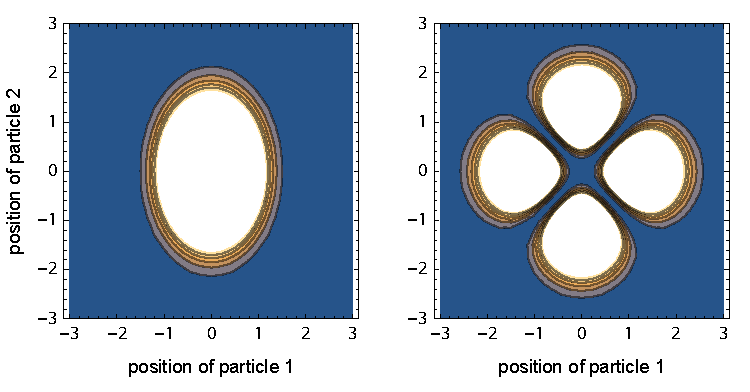
\includegraphics[center]{media/exchange}
\caption{\textbf{Antisymmetrization.}
Contour plots of the square of a wave function, $|\Psi(x_1,x_2)|^2$, of two particles in one dimension formed from two one-particle functions, $\phi_1(x)=\exp(-x^2)$ and $\phi_2(x)=\exp(-x^2/2)$.
On the left, $\Psi$ is a simple product.
On the right, $\Psi$ is an antisymmetrized product, $\phi_1(x_1)\phi_2(x_2)-\phi_1(x_2)\phi_2(x_1)$.
}\label{fig:exchange}
\end{figure}
